\documentclass[12pt]{article}   %using XeLatex for build it.
\usepackage{styles/packages}
\usepackage{styles/style}

% \CTEXsetup[format={\Large\bfseries}]{section} %设置Section左对齐。 ***** 用于中文设置。 *****

\begin{document}


\title{Probabilistic Systems Analysis and Applied Probability}
\author{Santiago}
\date{June 21, 2020}

\maketitle %渲染Title。

\begin{abstract}
	This course introduces students to the modeling, quantification, and analysis of uncertainty.  The tools of probability theory, and of the related field of statistical inference, are the keys for being able to analyze and make sense of data. These tools underlie important advances in many fields, from the basic sciences to engineering and management. \\
	Instructor(s) : Prof. John Tsitsiklis

\end{abstract}

\section{Lecture 1: Probability Models and Axioms}
    \subsection{Reading}
    \begin{itemize}
        \item Sections 1.1, 1.2
    \end{itemize}

    \subsection{Lecture outline}
    \begin{itemize}
        \item Probability as a mathematical framework for: 
        \begin{itemize}
            \item reasoning about uncertainty
            \item developing approaches to inference problems
        \end{itemize}

        \item Probabilistic models
        \begin{itemize}
            \item sample space
            \item probability law
        \end{itemize}

        \item Axioms of probability
        \item Simple examples
    \end{itemize}

    %% \texorpdfstring{$\Omega$}{} 这个是为了在标题中打印数学符号
    \subsection{Sample space \texorpdfstring{$\Omega$}{}}
    \begin{itemize}
        \item "List" (set) of possible outcomes
        \item List must be:
        \begin{itemize}
            \item Mutually exclusive(互斥)
            \item Collectively exhaustive(互补)
        \end{itemize}

        \item Art: to be at the "right" granularity(粒度)
    \end{itemize}

    \subsection{Sample space: Discrete example}
    \begin{itemize}
        \item Two rolls of a tetrahedral(四面體) die
        \begin{itemize}
            \item Sample space vs. sequential description
        \end{itemize}

        \item See Figure~\ref{fig:1-1}
		 
		 \begin{figure}[h!] % h for here.
		\centering
		 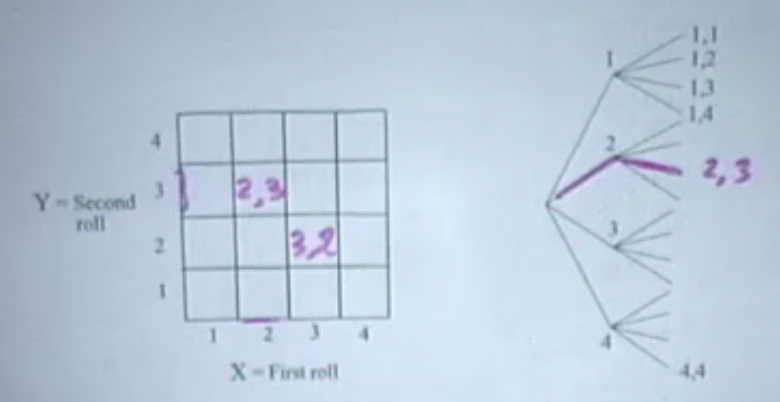
\includegraphics[scale=0.7]{images/1-1}
		\caption{Sample space: Discrete example}
		 \label{fig:1-1}
		 \end{figure}
    \end{itemize}

    \subsection{Sample space: Continuous example}
    \begin{itemize}
        \item $\omega = \{(x,y) | 0 \le x,y \le 1\}$
        \item See Figure~\ref{fig:1-2}
		 
        \begin{figure}[h!] % h for here.
       \centering
        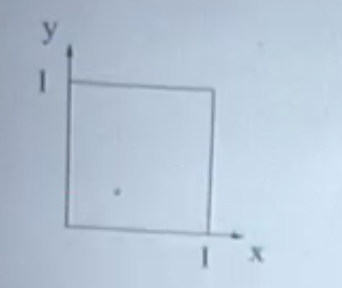
\includegraphics[scale=0.7]{images/1-2}
       \caption{Sample space: Continuous example}
        \label{fig:1-2}
        \end{figure}
    \end{itemize}

    \subsection{Probability axioms(公理)}
    \begin{itemize}
        \item \textbf{Event:} a subset of the sample space
        \item See Figure~\ref{fig:1-3}
		 
        \begin{figure}[h!] % h for here.
       \centering
        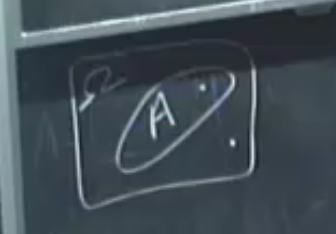
\includegraphics[scale=0.7]{images/1-3}
       \caption{Event: a subset of the sample space}
        \label{fig:1-3}
        \end{figure}

        \item Probability is assigned to events
        
        \rule{\textwidth}{1pt} %横线
        \item \textbf{Axioms:}
        \item 1. \textbf{Nonnegativity:} $P(A) \geq 0$
        \item 2. \textbf{Normalization:} $P(\Omega) = 1$
        \item 3. \textbf{Additivity:} If $A \cap B = \emptyset$, then $P(A \cup B) = P(A)+ P(B)$
        \rule{\textwidth}{1pt} %横线

        \item See Figure~\ref{fig:1-4}
		 
        \begin{figure}[h!] % h for here.
       \centering
        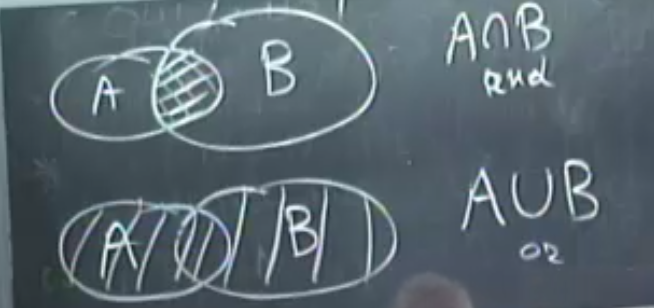
\includegraphics[scale=0.7]{images/1-4}
       \caption{Axioms: Additivity}
        \label{fig:1-4}
        \end{figure}
            
        \begin{eqnarray*}
            1 & \overset{(2)}{=} & P(\Omega) = P(A \cup A^c) \\
            & \overset{(3)}{=} & P(A) + P(A^c) \\
            P(A) & = & 1 - P(A^c) \overset{(1)}{\leq} 1
        \end{eqnarray*}

        \item See Figure~\ref{fig:1-5}
        \begin{figure}[h!]
            \centering
            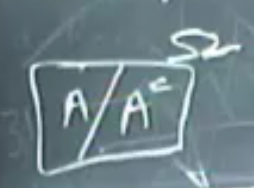
\includegraphics[scale=0.7]{images/1-5}
            \caption{A and complement of A}
            \label{fig:1-5}
        \end{figure}

        \begin{eqnarray*}
            && P(A \cup B \cup C) \\
            && = P((A \cup B) \cup C) \\
            && = P(A \cup B) + P(C) \\
            && = P(A) + P(B) + P(C)
        \end{eqnarray*}

        If $A_1,A_2,...,A_n$ disjoint.
        the $P(A_1 \cup ... \cup A_n) = P(A_1)+...+P(A_n)$

        \item See Figure~\ref{fig:1-6}
        \begin{figure}[h!]
            \centering
            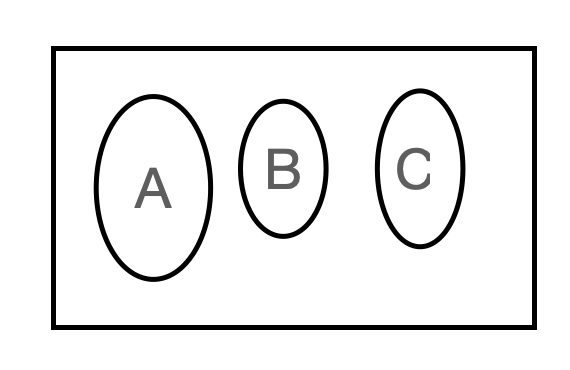
\includegraphics[scale=0.7]{images/1-6}
            \caption{A,B,C in an $Omega$}
            \label{fig:1-6}
        \end{figure}

        \begin{eqnarray*}
            P(\{s_1, s_2, \dots, s_k\}) & = & P(\{s_1\}) + \dots + P(\{s_k\}) \\
            & = & P(s_1) + \dots + P(s_k)
        \end{eqnarray*}

        \item See Figure~\ref{fig:1-7}
        \begin{figure}[h!]
            \centering
            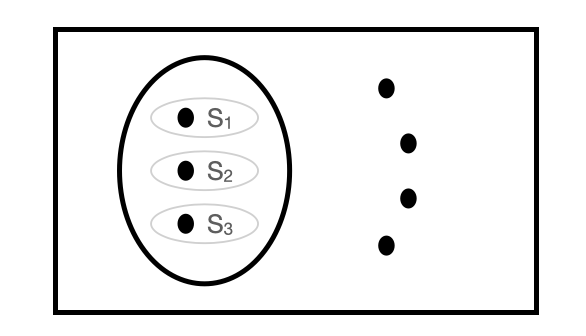
\includegraphics[scale=0.7]{images/1-7}
            \caption{finite elements in an $Omega$}
            \label{fig:1-7}
        \end{figure}


        \item Axiom 3 needs strengthening(加强)
        \item Do weird sets have probabilities?
        
    \end{itemize}

\subsection{Probability law: Example with finite sample space}
    \begin{itemize}
        \item See Figure~\ref{fig:1-8}
        \begin{figure}[h!]
            \centering
            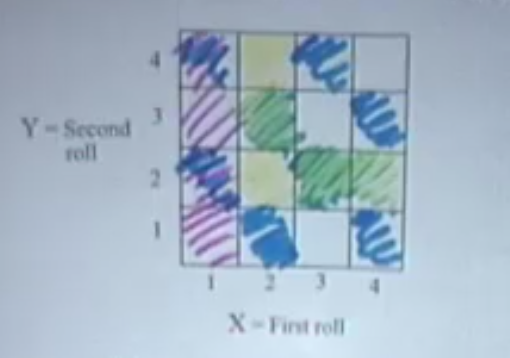
\includegraphics[scale=0.7]{images/1-8}
            \caption{Probability law: Example with finite sample space}
            \label{fig:1-8}
        \end{figure}
        
        \item Let every possible outcome have probability 1/16
        \begin{itemize}
            \item $ P((X,Y) \; is \; (1,1) \; or \; (1,2)) = 2/16$
            \item $ P({X=1}) =  4/16$
            \item $ P(X+Y \; is \; odd) = 8/16$
            \item $ P(min(X,Y)=2) = 5/16$
        \end{itemize}
    \end{itemize}

\subsection{Discrete uniform law}
    \begin{itemize}
        \item Let all outcomes be equally likely
        \item Then, 
        $$
        P(A) = \frac{number \; of \; elements \; of \; A}{total  \; number \; of \; sample \; points}
        $$
        \item Computing probabilities $\equiv$ counting
        \item Defines fair coins, fair dice, well-shuffled card decks
    \end{itemize}

\subsection{Continuous uniform law}
    \begin{itemize}
        \item Two "random" numbers is [0,1].
        \item See Figure~\ref{fig:1-9}
        \begin{figure}[h!]
            \centering
            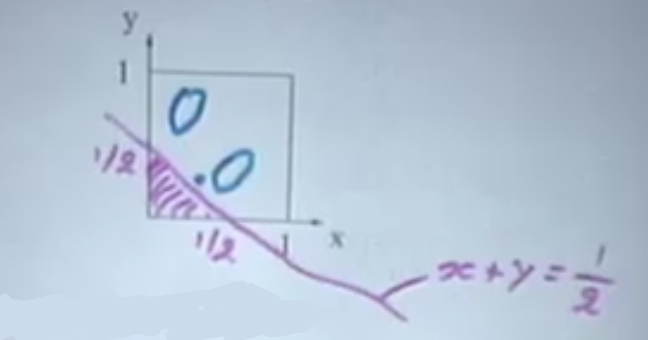
\includegraphics[scale=0.7]{images/1-9}
            \caption{Continuous uniform law}
            \label{fig:1-9}
        \end{figure}
        \item \textbf{Uniform} law: Probability \equiv Area 
        \begin{itemize}
            \item $P(X+Y \leq 1/2) = \frac{1}{2} \cdot \frac{1}{2} \cdot \frac{1}{2} = \frac{1}{8}$
            \item $P((X,Y)=(0.5, 0.3)) = 0$
        \end{itemize}
    \end{itemize}

\subsection{Probability law: Ex. w/countably infinite sample space}
    \begin{itemize}
        \item Sample space: $\{1,2,...\}$
        \begin{itemize}
            \item We are given $P(n) = 2^{-n}, n=1,2,...$
            \item Find $P(outcome \; is \; even)$
            \item See Figure~\ref{fig:1-10}
            \begin{figure}[h!]
                \centering
                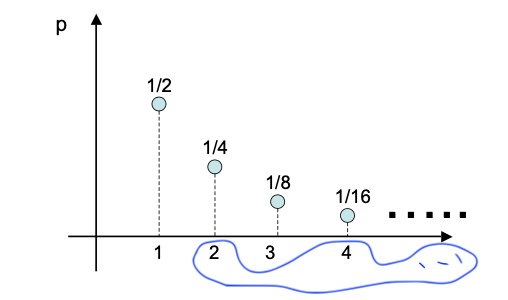
\includegraphics[scale=0.7]{images/1-10}
                \caption{Probability law: Ex. w/countably infinite sample space}
                \label{fig:1-10}
            \end{figure}
            $$
            P(\{2,4,6,...\}) = P(2) + P(4) + ... = \frac{1}{2^2} + \frac{1}{2^4} + \frac{1}{2^6}
            $$
        \end{itemize}

        \item Countable Additivity axiom (needed for this calculation)(Santiago comment: It is \textbf{infinite} on this example instead of finite on before one ): \\
        If $A_1, A_2, ...$ are disjoint events, then:
        $$
        P(A_1 \cup A_2 \cup ...) = P(A_1) + P(A_2) + ...
        $$
        
    \end{itemize}



\section{Week 666666 - Transport Layer Overview}
	{\color{pink} dddd}


\end{document}

